\documentclass[mathserif]{beamer}
\usepackage{epstopdf}
\usepackage{helvet}
\usecolortheme{beaver}

\usepackage[brazil]{babel}
\usepackage[utf8]{inputenc}


\title{\textbf{Simulação de Esquemas \\ de Modulação Digital}}
%\subtitle{Subtitle}
\author{David Anchieta \\ Arthur Ramos \\ Hanna Vitória \\ Itamar de Aguiar}


\begin{document}
	\frame{\titlepage}

	\begin{frame}{BPSK}
		\begin{figure}
			\centering
			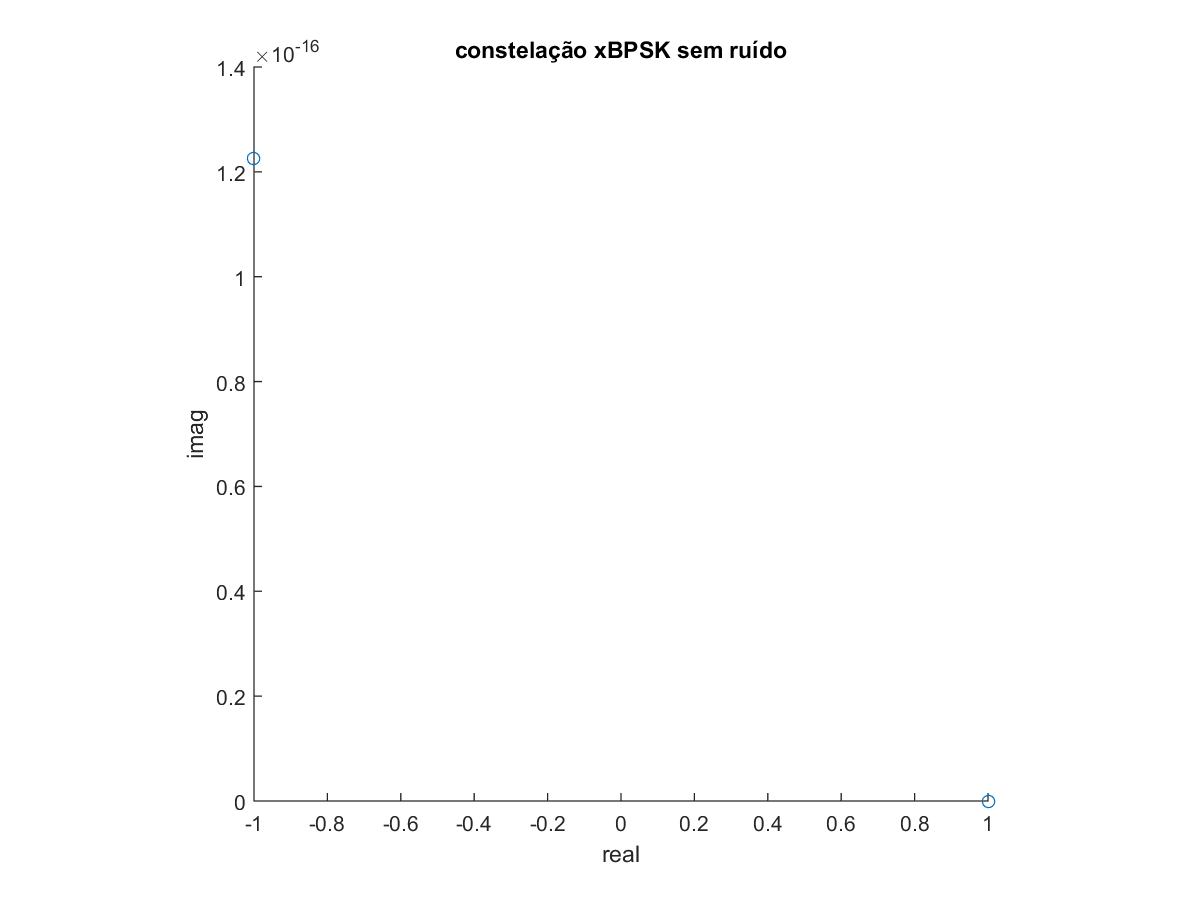
\includegraphics[scale=0.3]{../NossoCodigo2/figuras/modula1.png}
			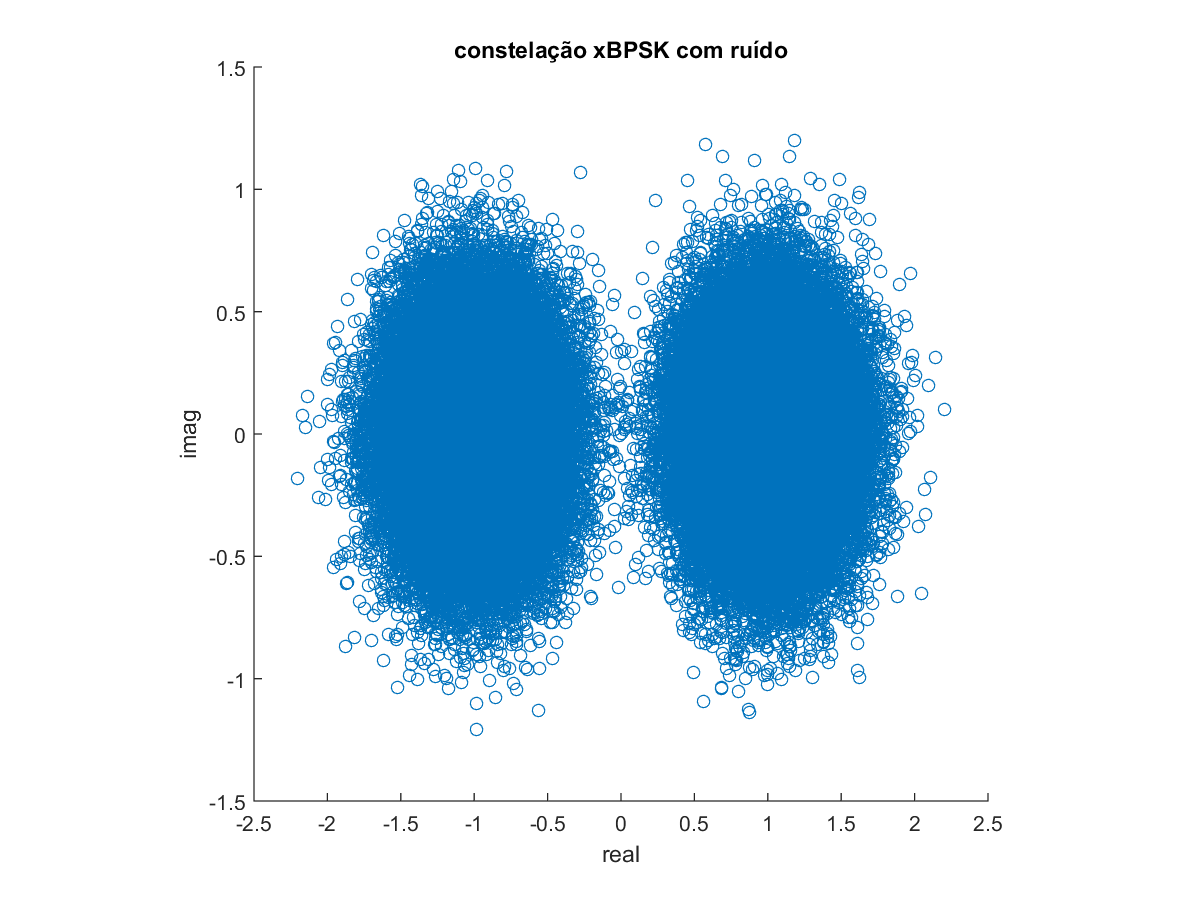
\includegraphics[scale=0.3]{../NossoCodigo2/figuras/modula7.png}
			%\caption{}
		\end{figure}
	\end{frame}

	\begin{frame}{QPSK}
		\begin{figure}
			\centering
			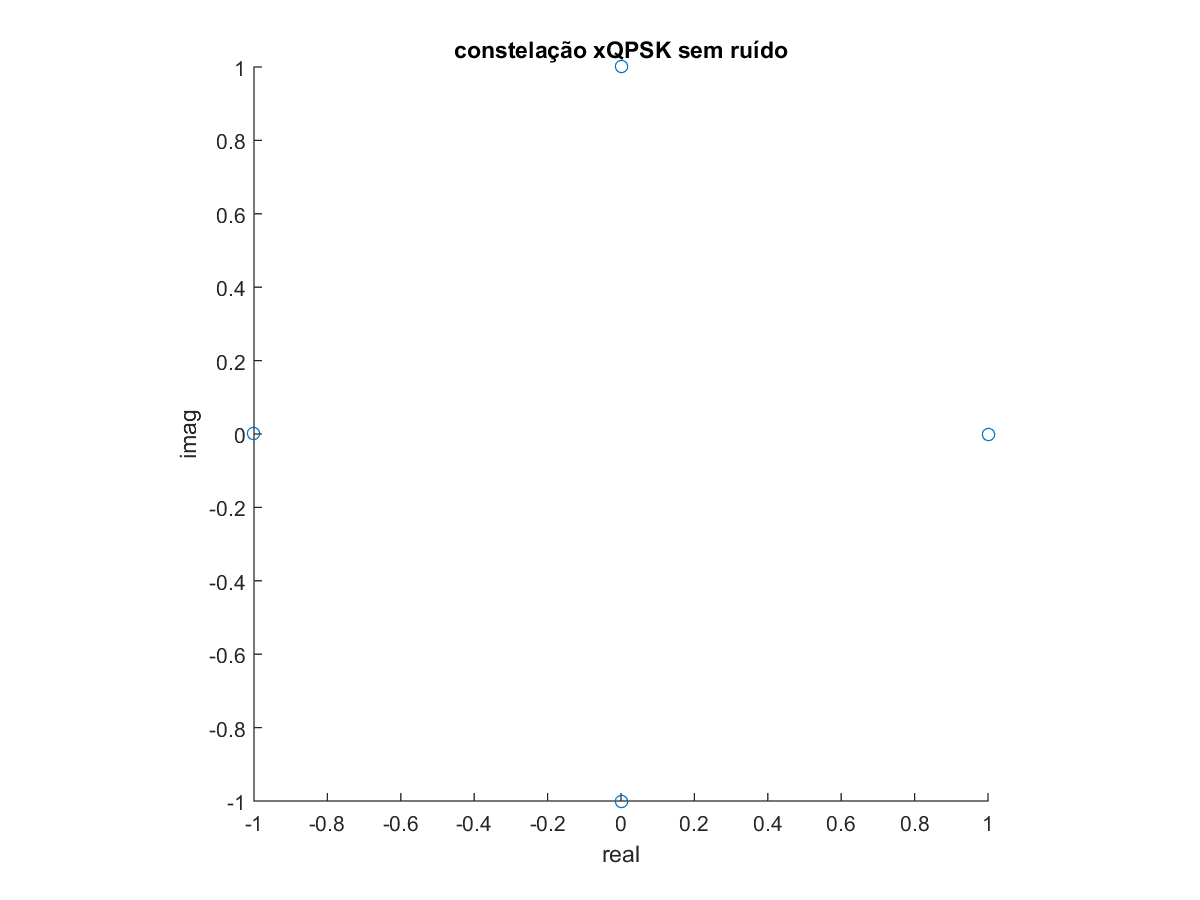
\includegraphics[scale=0.3]{../NossoCodigo2/figuras/modula2.png}
			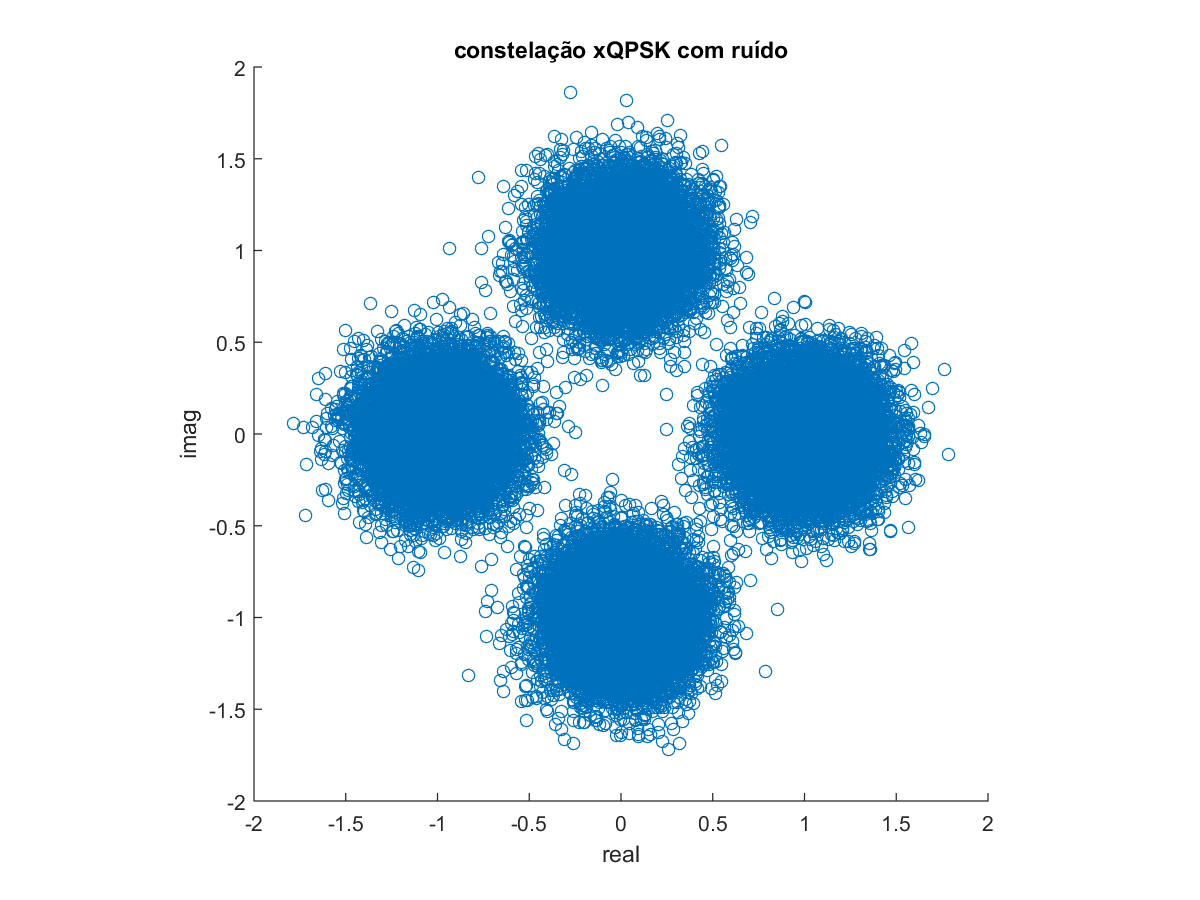
\includegraphics[scale=0.3]{../NossoCodigo2/figuras/modula8.png}
			%\caption{}
		\end{figure}
	\end{frame}

	\begin{frame}{PSK 8}
		\begin{figure}
			\centering
			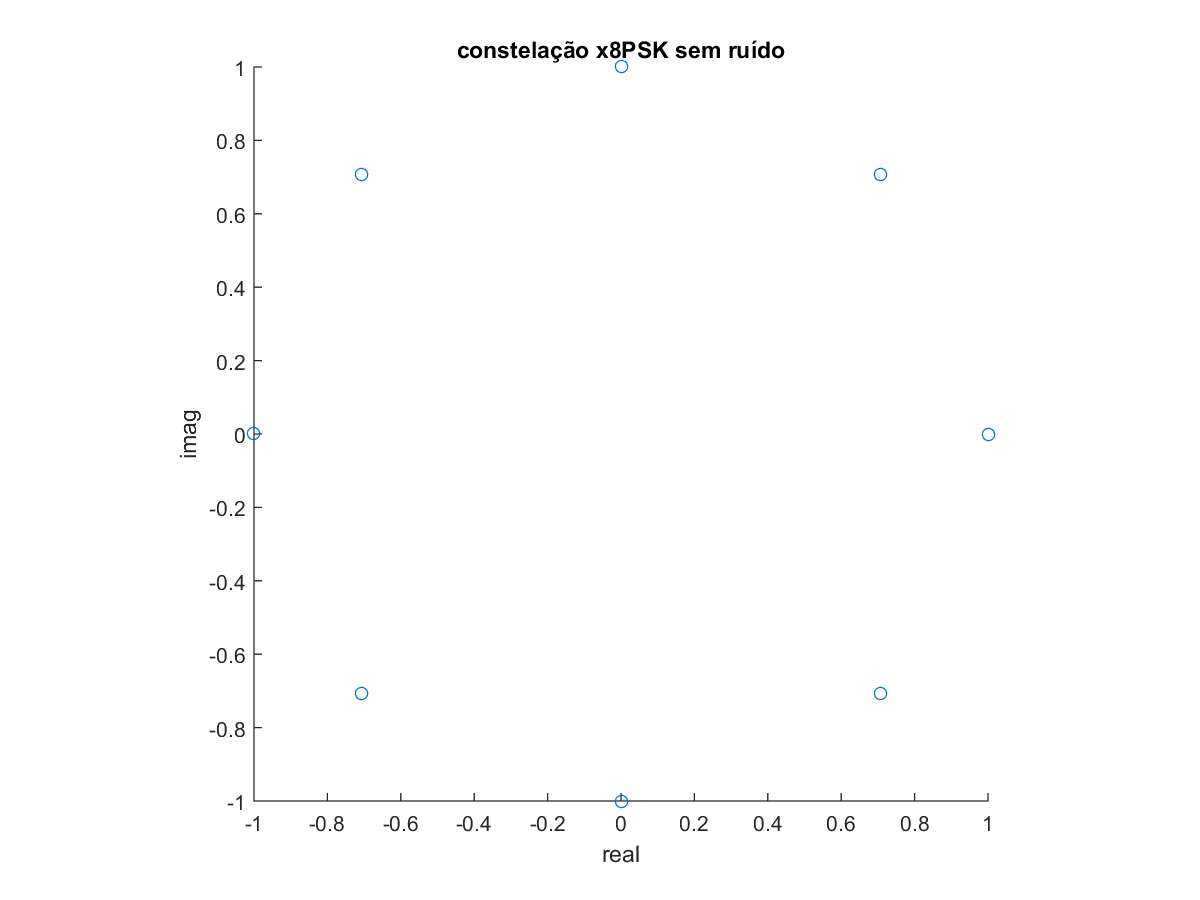
\includegraphics[scale=0.3]{../NossoCodigo2/figuras/modula3.png}
			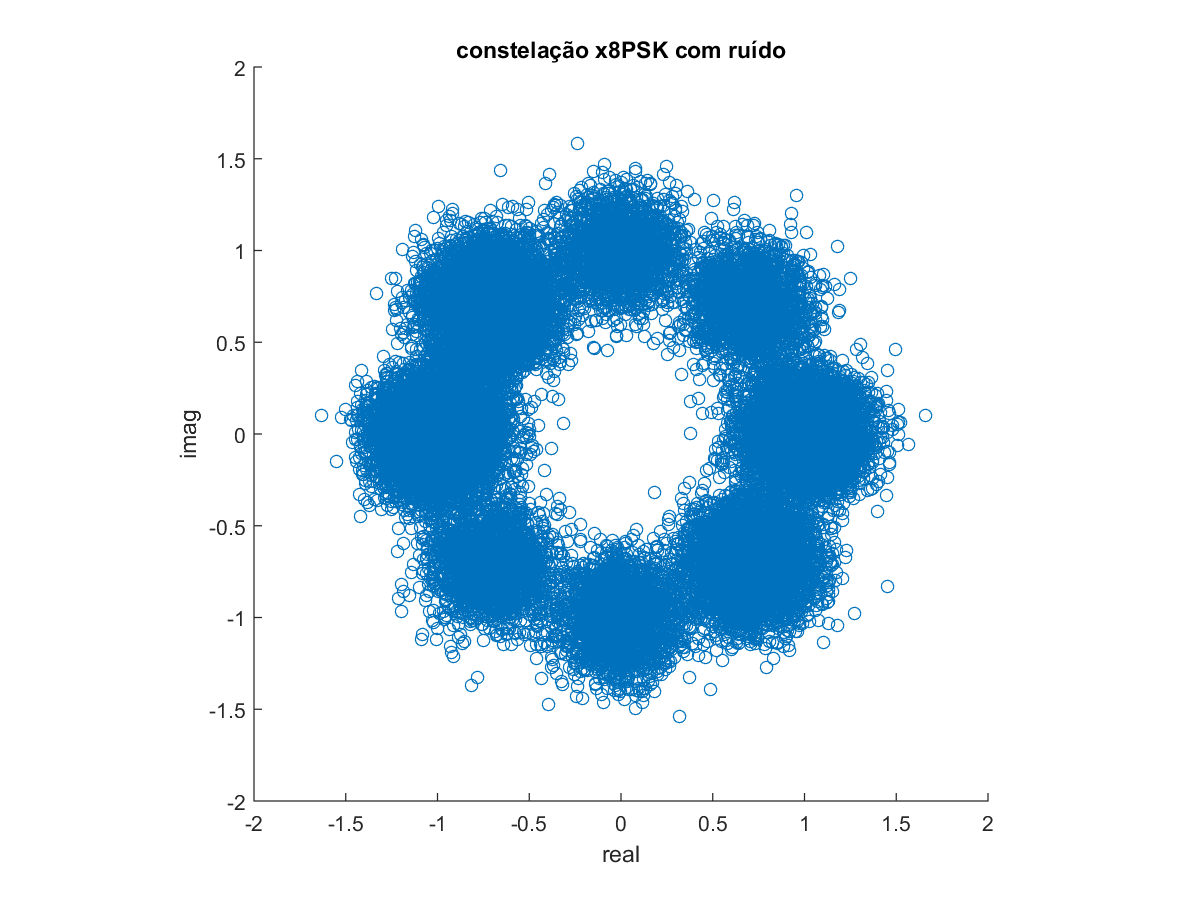
\includegraphics[scale=0.3]{../NossoCodigo2/figuras/modula9.png}
			%\caption{}
		\end{figure}
	\end{frame}

	\begin{frame}{PSK 16}
		\begin{figure}
			\centering
			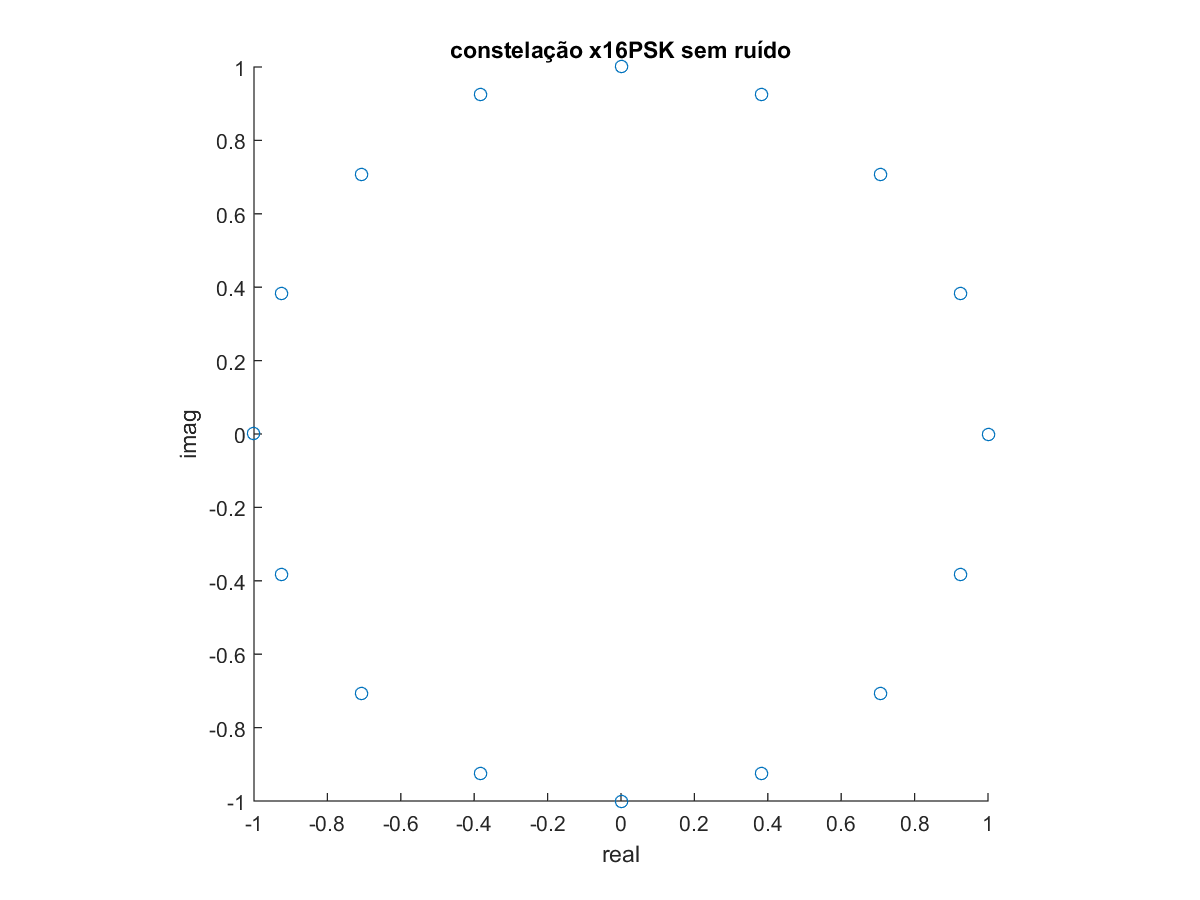
\includegraphics[scale=0.3]{../NossoCodigo2/figuras/modula4.png}
			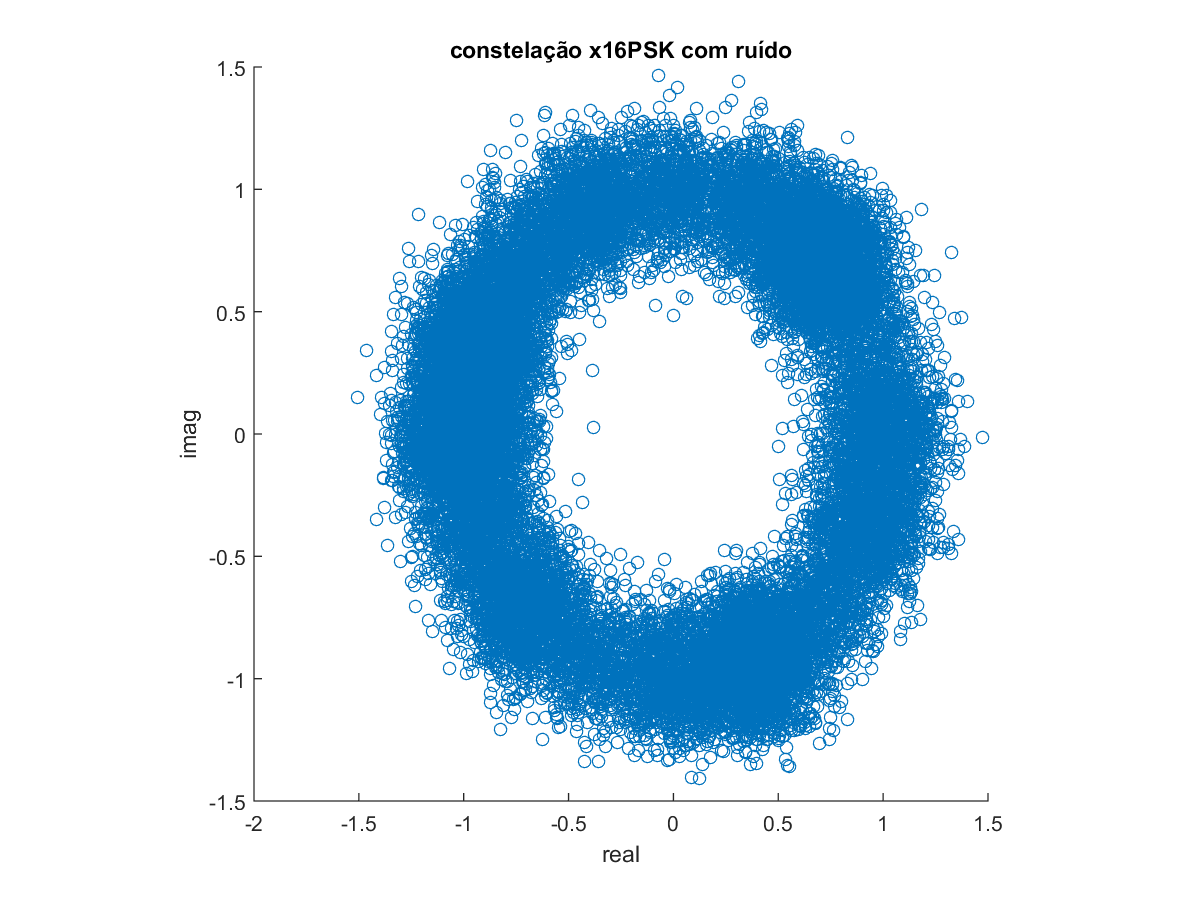
\includegraphics[scale=0.3]{../NossoCodigo2/figuras/modula10.png}
			%\caption{}
		\end{figure}
	\end{frame}

	\begin{frame}{QAM}
		\begin{figure}
			\centering
			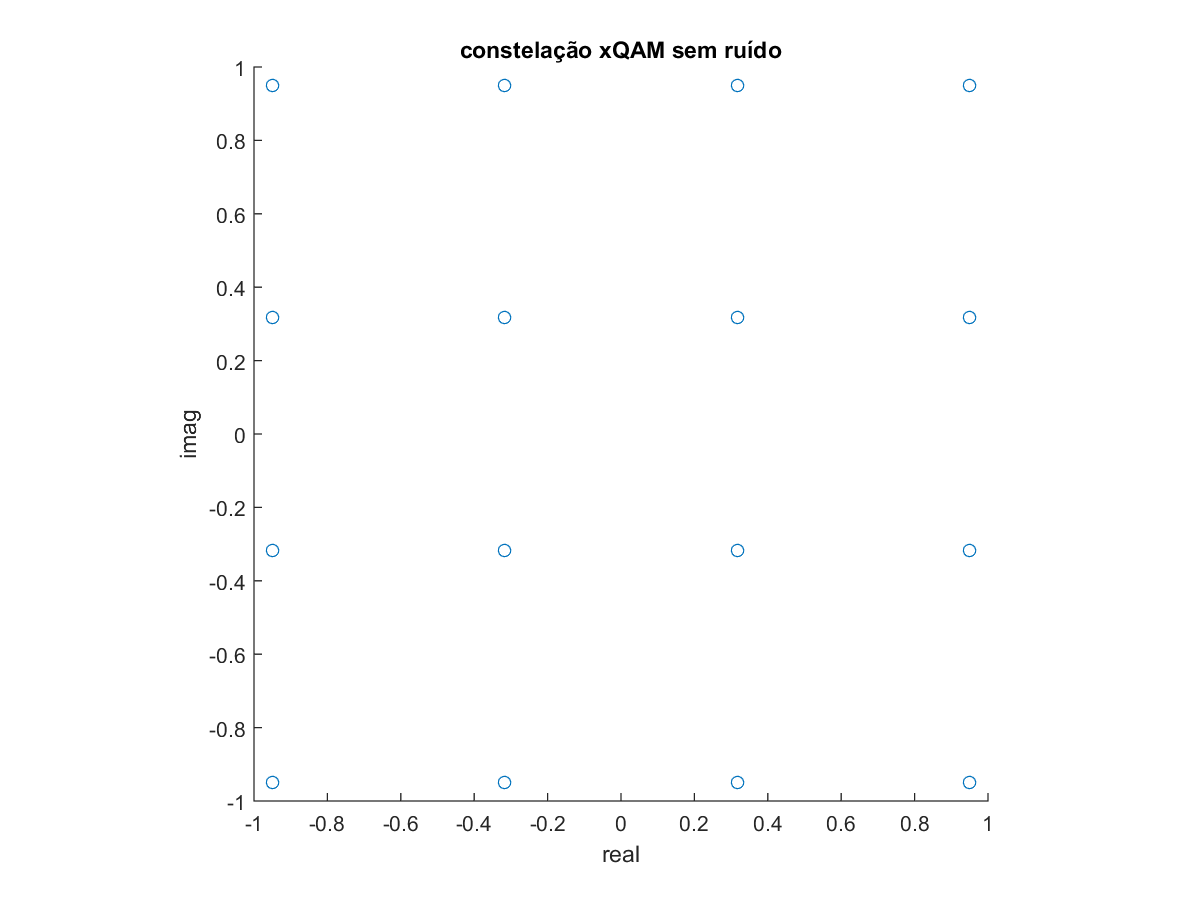
\includegraphics[scale=0.3]{../NossoCodigo2/figuras/modula6.png}
			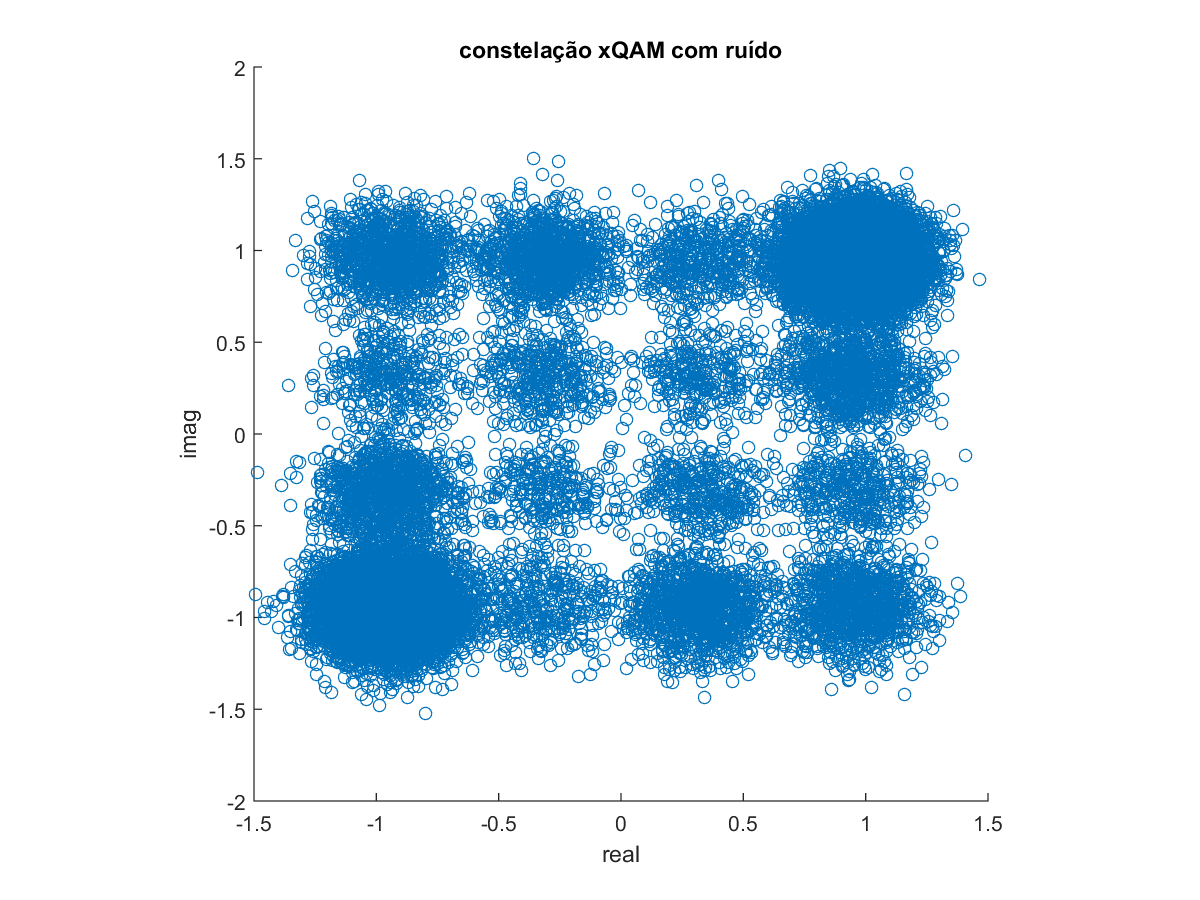
\includegraphics[scale=0.3]{../NossoCodigo2/figuras/modula12.png}
			%\caption{}
		\end{figure}
	\end{frame}

	\begin{frame}{Taxa de erro de bits}
		BER BPSK = 2.4085e-04


		BER QPSK = 1.9067e-04


		BER 8PSK = 0.0122


		BER 16PSK = 0.0808


		BER QAM = 0.0379
	\end{frame}

	\begin{frame}{Largura de banda}
		BPSK = 49152 Hz


		BER QPSK = 24576 Hz


		BER 8PSK = 16384 Hz


		BER 16PSK = 12288 Hz


		BER QAM = 12288 Hz
		
	\end{frame}
	

	\begin{frame}{BPSK}
		\begin{figure}
			\centering
			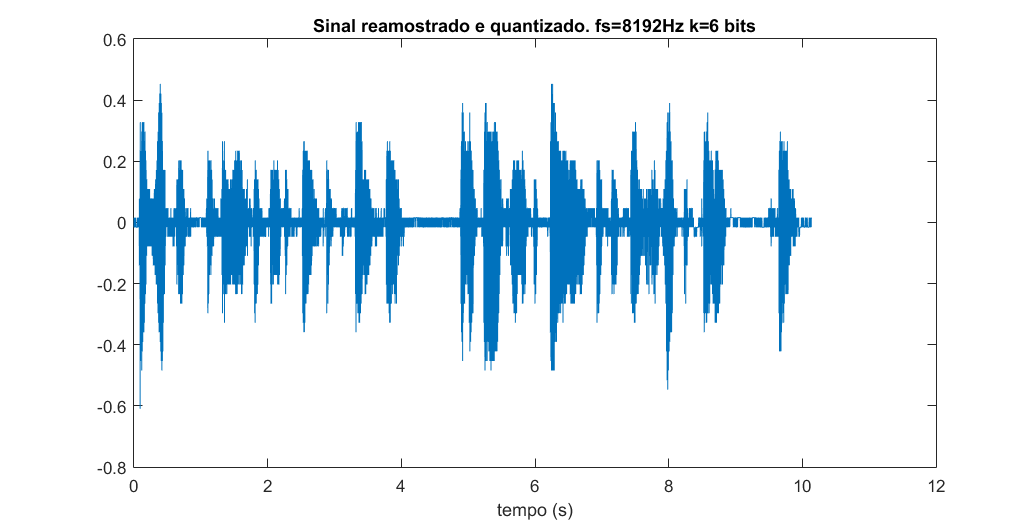
\includegraphics[scale=0.3]{../NossoCodigo2/figuras/0quantizado.png}
			\quad
			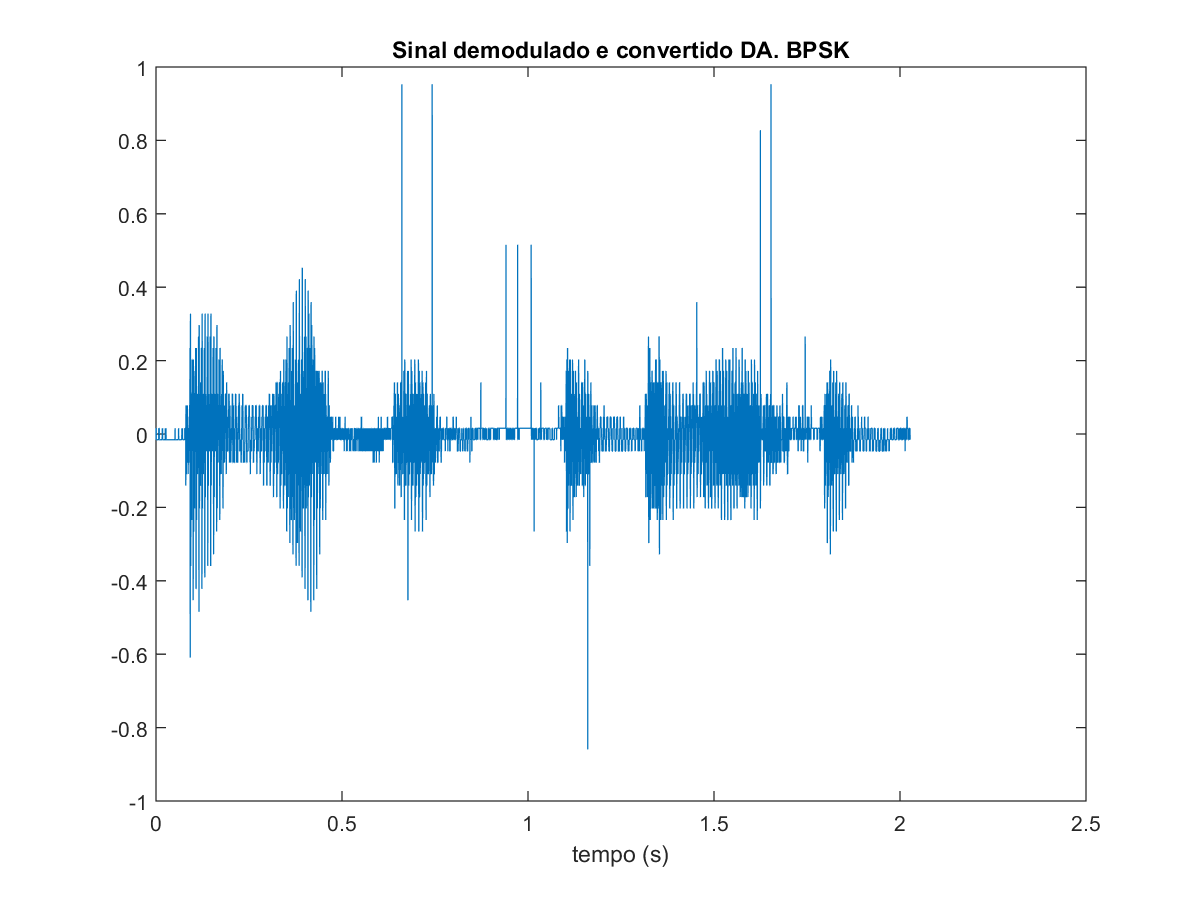
\includegraphics[scale=0.3]{../NossoCodigo2/figuras/modula13.png}
			%\caption{}
		\end{figure}
	\end{frame}

	\begin{frame}{QPSK}
		\begin{figure}
			\centering
			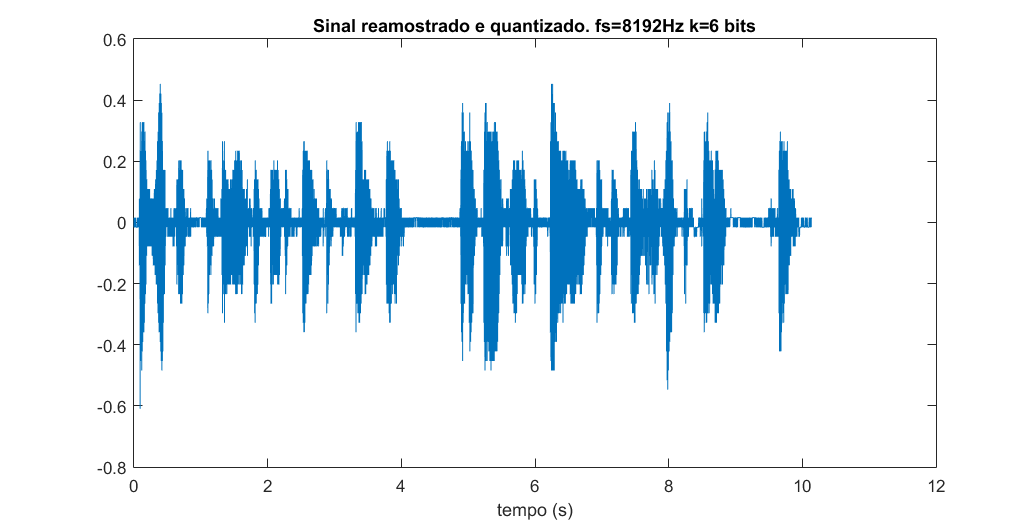
\includegraphics[scale=0.3]{../NossoCodigo2/figuras/0quantizado.png}
			\quad
			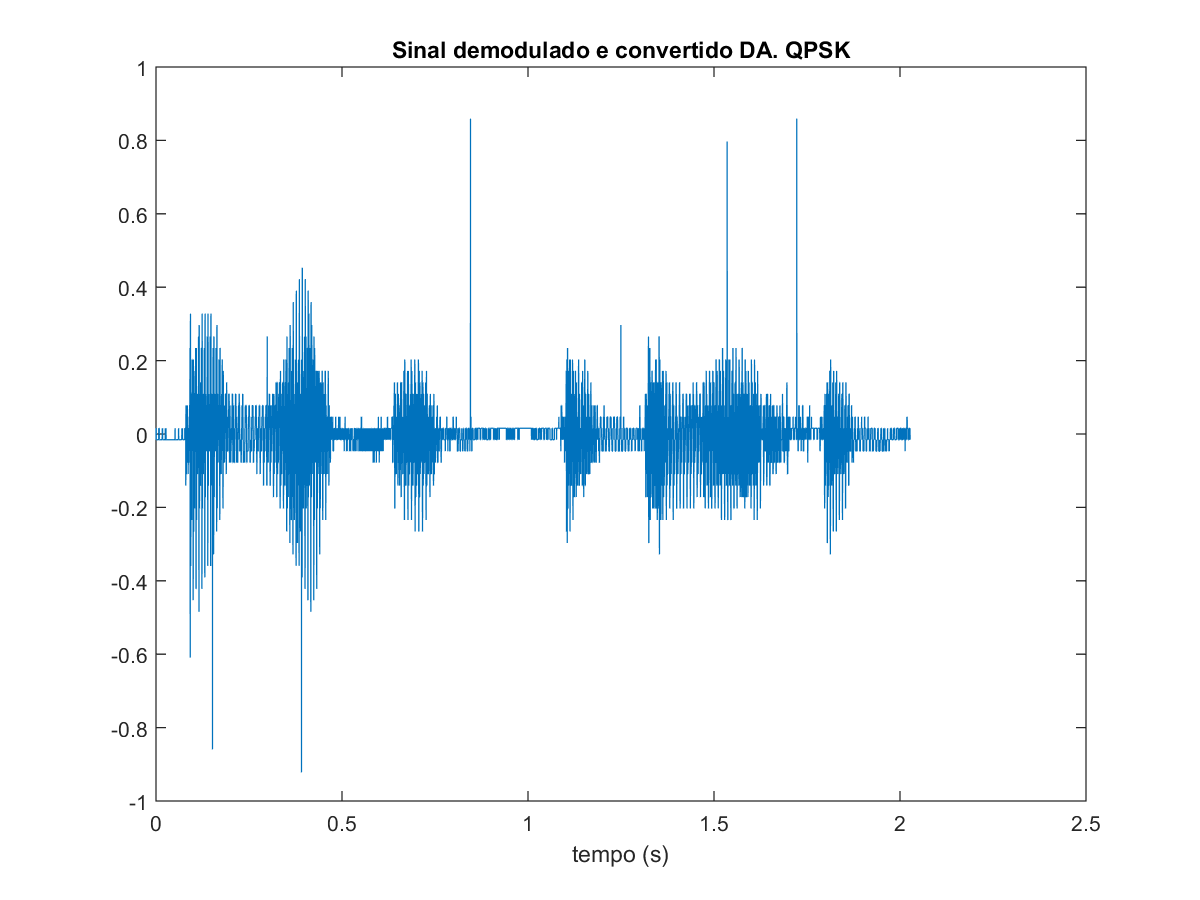
\includegraphics[scale=0.3]{../NossoCodigo2/figuras/modula14.png}
			%\caption{}
		\end{figure}
	\end{frame}

	\begin{frame}{8PSK}
		\begin{figure}
			\centering
			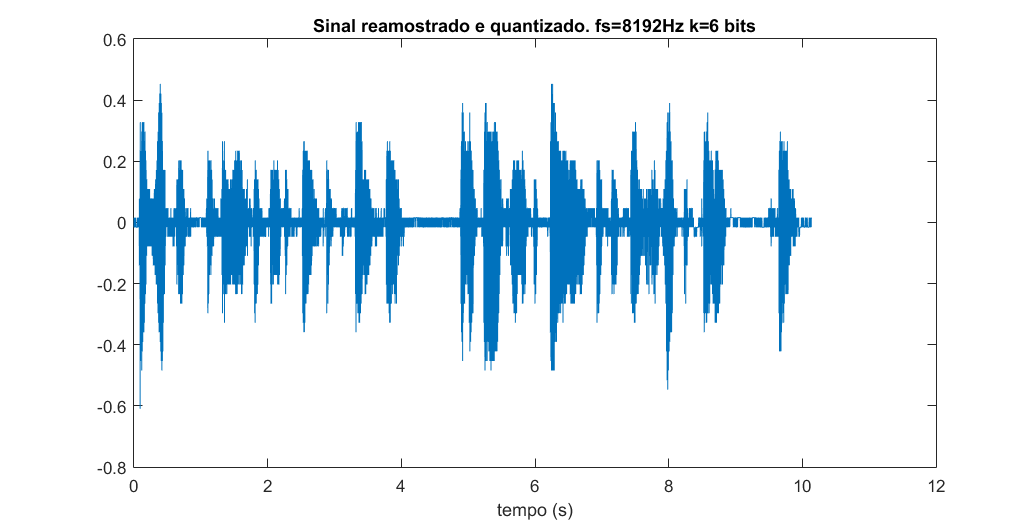
\includegraphics[scale=0.3]{../NossoCodigo2/figuras/0quantizado.png}
			\quad
			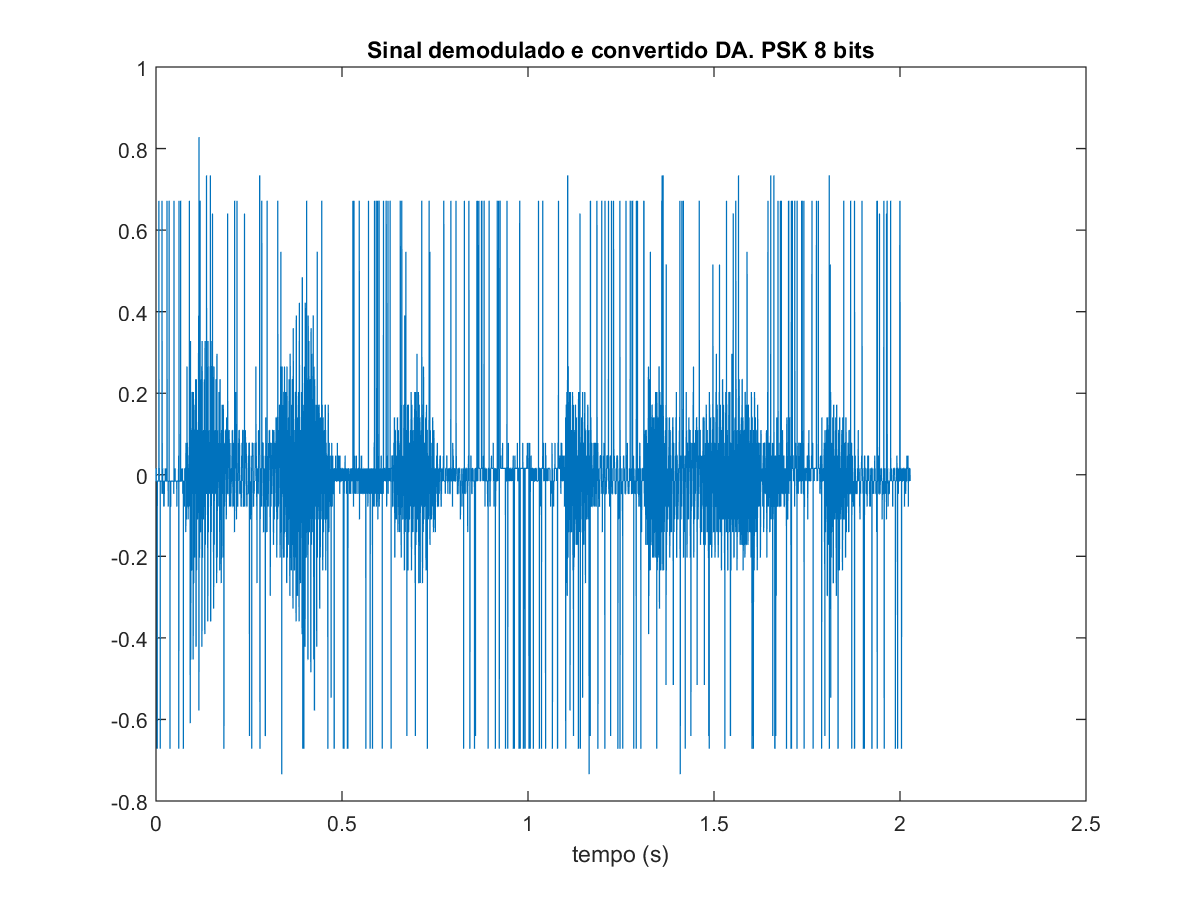
\includegraphics[scale=0.3]{../NossoCodigo2/figuras/modula15.png}
			%\caption{}
		\end{figure}
	\end{frame}

	\begin{frame}{16PSK}
		\begin{figure}
			\centering
			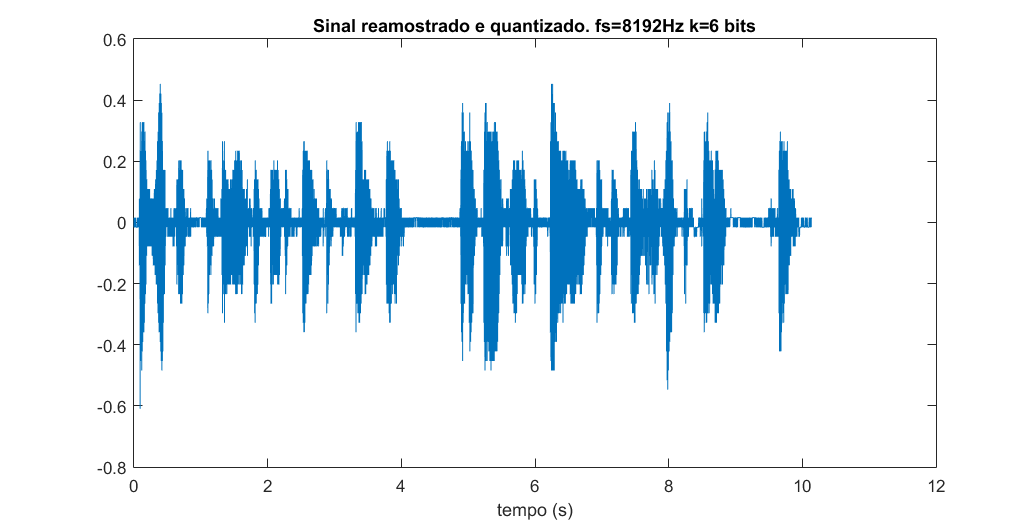
\includegraphics[scale=0.3]{../NossoCodigo2/figuras/0quantizado.png}
			\quad
			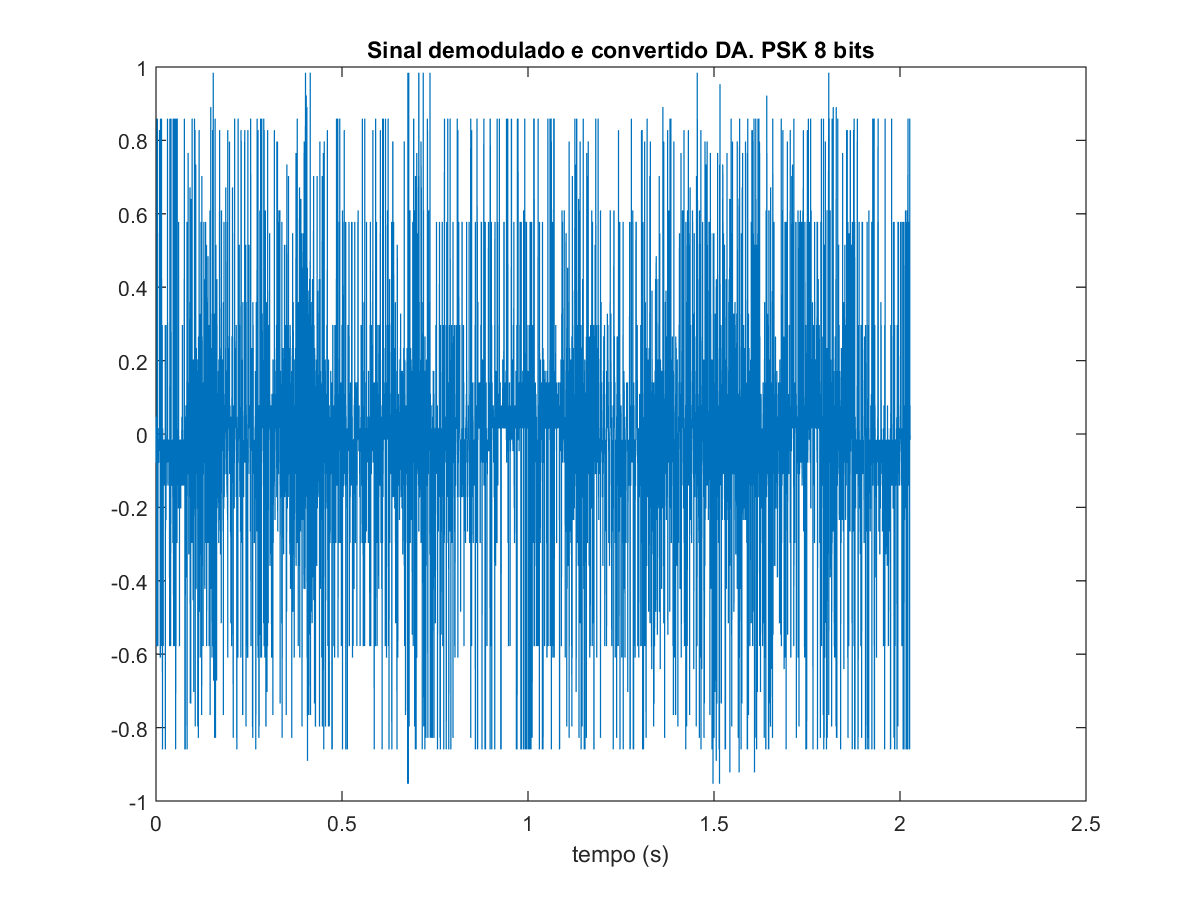
\includegraphics[scale=0.3]{../NossoCodigo2/figuras/modula16.png}
			%\caption{}
		\end{figure}
	\end{frame}

	\begin{frame}{QAM}
		\begin{figure}
			\centering
			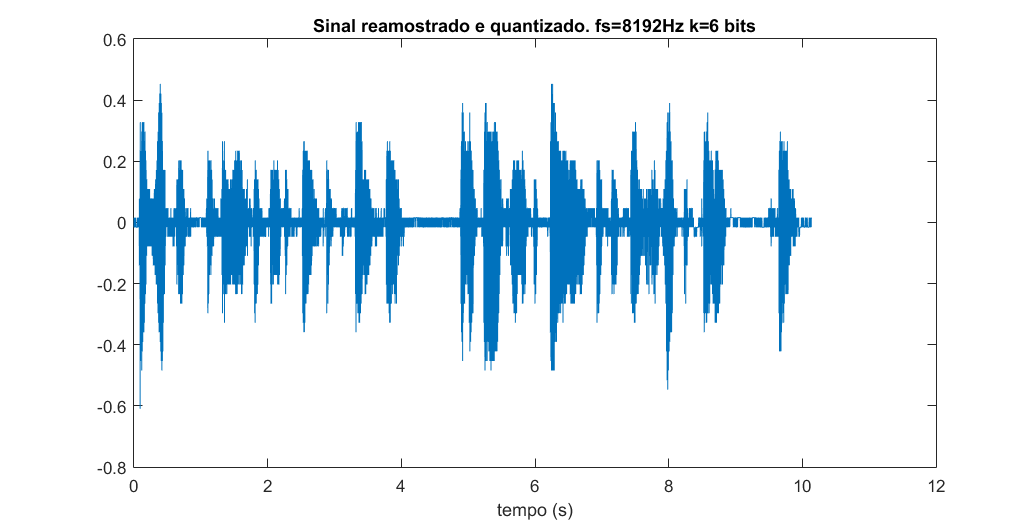
\includegraphics[scale=0.3]{../NossoCodigo2/figuras/0quantizado.png}
			\quad
			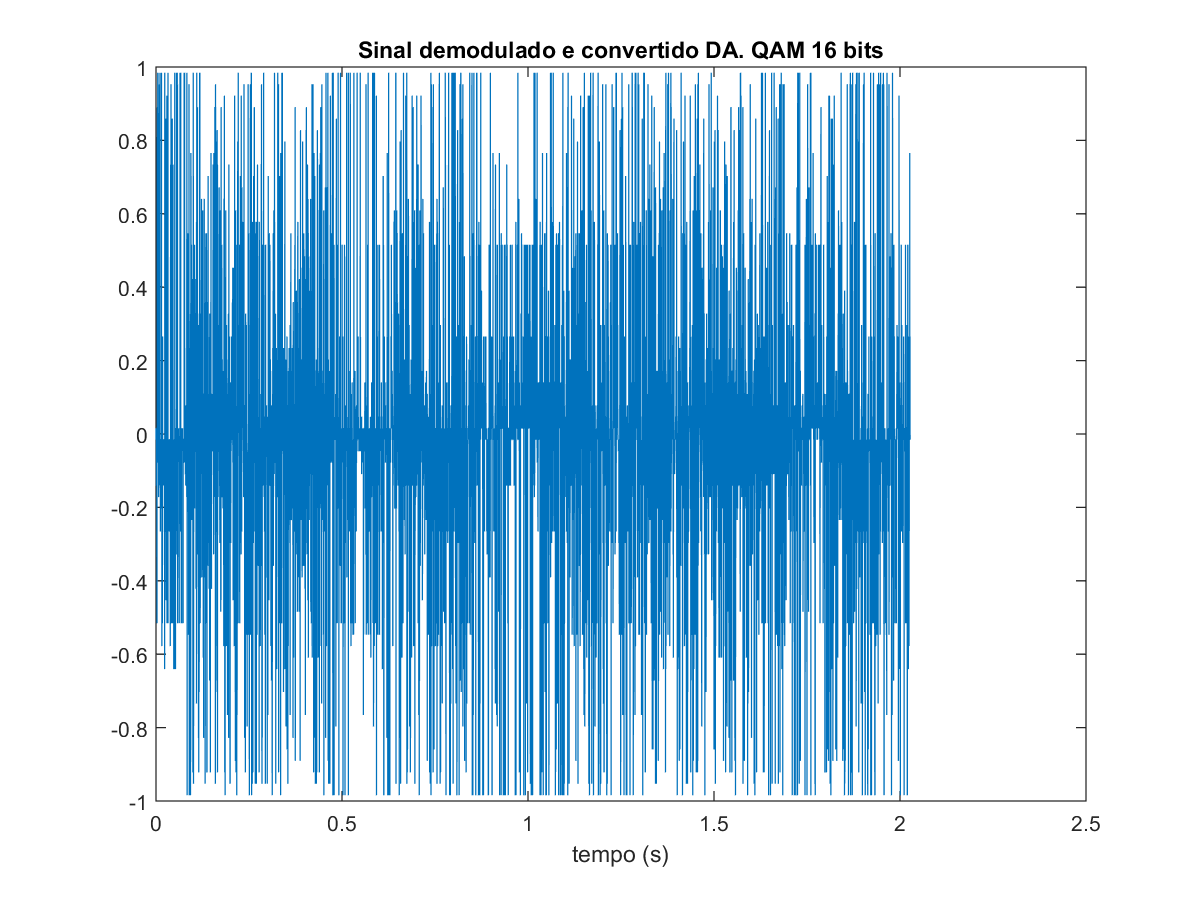
\includegraphics[scale=0.3]{../NossoCodigo2/figuras/modula18.png}
			%\caption{}
		\end{figure}
	\end{frame}

	\begin{frame}{Qualidade de áudio}
		\begin{enumerate}
		\item BPSK (quase igual ao original)
		\item QAM 16 bits (Melhor custo/benefício)
		\item QPSK
		\item PSK 8 
		\item PSK 16
		\end{enumerate}

	\end{frame}
	


	
\end{document}